\documentclass[useAMS,usenatbib]{mn2e}
%\documentclass[twocolumn]{emulateapj}
\usepackage{graphicx,natbib,color,multirow,amsmath}
\voffset=-0.8in

\definecolor{titlecol}{rgb}{0,0,1}
\definecolor{titlecol2}{rgb}{0,0.65,0}
\definecolor{titlecol3}{rgb}{0.99,0.4,0.}

%\definecolor{titledark}{rgb}{0,0,0.8}
%\definecolor{hilit}{rgb}{0,0,1}
%\definecolor{hilitdark}{rgb}{0,0,0.8}
%\font\sbf=cmssbx10 at 32.28pt %big font for headers

\font\nbf=cmssbx10 at 12.28pt %big font for headers

%%%%%%%%%%%%%%%%%%%%%%%%%%%%%%%
%%%% If you want to leave notes in the text feel free to define
%%%% your own colour above and a style below
%%%%%%%%%%%%%%%%%%%%%%%%%%%%%%%
\def\note		{\color{titlecol2} \nbf}
\def\noteb		{\color{titlecol} \nbf}
\def\notebsm	{\color{titlecol}}
\def\notec		{\color{titlecol2} \nbf}
\def\notecsm	{\color{titlecol2}}
\def\notek		{\color{titlecol3} }

%%%%%%%%%%%%%%%%%%%%%%%%%%%%%%%
% For the eventual referee response
\def\changed    {\color{titlecol} }
%\def\changed    {}


%%%%%%%%%%%%%%%%%%%%%%%%%%%%%%%
%  Other stuff I use a lot
\def\oiii		{$\mathrm{\left[ O \textsc{iii}\right] }$}
\def\moiii		{\mathrm{\left[ O \textsc{iii}\right] }}
\def\nii		{$\mathrm{\left[ N \textsc{ii}\right] }$}
\def\mnii		{\mathrm{\left[ N \textsc{ii}\right] }}
\def\sii		{$\mathrm{\left[ S \textsc{ii}\right] }$}
\def\msii		{\mathrm{\left[ S \textsc{ii}\right] }}
\def\galfit     {{\tt GALFIT}}

\def\mmsun	{\rm{M}_{\odot}}
\def\fnobulge    {$f_{\rm no~bulge}$}
\def\mfnobulge {f_{\rm no~bulge}}
\def\fedgeon     {$f_{\rm edge-on}$}
\def\mfedgeon  {f_{\rm edge-on}}
\def\fcnobulge    {$f_{\rm confirmed~no~bulge}$}
\def\mfcnobulge {f_{\rm confirmed~no~bulge}}


%\def\lesssim{\mathrel{\hbox{\rlap{\hbox{\lower5pt\hbox{$\sim$}}}\hbox{$<$}}}}
%\def\gtrsim{\mathrel{\hbox{\rlap{\hbox{\lower5pt\hbox{$\sim$}}}\hbox{$>$}}}}
%new defs of lesssim gtrsim that I think look better
\def\lesssim{\mathrel{\hbox{\rlap{\hbox{\lower3pt\hbox{$\sim$}}}\hbox{\raise2pt\hbox{$<$}}}}}
\def\gtrsim{\mathrel{\hbox{\rlap{\hbox{\lower3pt\hbox{$\sim$}}}\hbox{\raise2pt\hbox{$>$}}}}}


\newcommand\nodata{ ~$\cdots$~ }




\begin{document}

\title[Galaxy Zoo-CANDELS : Bar Fractions from $0.5 < z < 2$]{Galaxy Zoo-CANDELS : Bar Fractions from $0.5 < z < 2$\thanks{This publication has been made possible by the participation of more than 200,000 volunteers in the Galaxy Zoo project. Their contributions are
individually acknowledged at http://authors.galaxyzoo.org/ .} } 

\author[Simmons et al.]{\parbox[t]{16cm}{{\notebsm B. D. Simmons$^{1}\thanks{E-mail: brooke.simmons@astro.ox.ac.uk}$}, 
%% Melvin did analysis & wrote introduction & provided comments & discussion
Thomas Melvin$^{2}$, 
%% Lintott & Masters provided substantial input & comments + many discussions
%% The order of these two is really difficult.
Chris Lintott$^{1}$, 
Karen Masters$^{2,3}$, 
%% Note Masters, Melvin, Willett, Keel, Rutkowski, Schawinski, Smethurst, Cheung all provided bar classifications
%% Schawinski's were tragically lost during a bugged-code incident, but they were submitted nonetheless.
%% Also Masters, Melvin, Willett, Keel, Schawinski, Smethurst, Cheung have all given comments on drafts.
%% This sub-list is not in any particular order at the moment.
{\notek Kyle W. Willett$^{4}$}, 
William C. Keel$^{X}$, 
Rebecca Smethurst$^{1}$, 
Edmond Cheung$^{X}$, 
%% Have had discussions with Bob that were really helpful as well as written comments - doesn't seem right to put him below 
%% all 8 who submitted 876 classifications apiece, though they should be high too. 
Robert C. Nichol$^{X}$, 
Kevin Schawinski$^{X}$, 
Michael Rutkowski$^{X}$,
%% Jeyhan made the color images for GZ
{\notec Jeyhan Kartaltepe$^{X, H}$,}
%% Conselice, Mortlock, Hartley, Almaini are citations for inclusion of unpublished UDS specz and photoz data
%% Others are core/data builders in CANDELS or were on telecons or sent comments to me
{\notec Christopher Conselice$^{X}$,}
{\notec Alice Mortlock$^{X}$, }
{\notec William Hartley$^{X}$,}
{\notec Omar Almaini $^{X}$,}
{\notec Eric Bell$^{X}$,}
Kevin R. V. Casteels$^{X}$, 
{\notec Dale Kocevski$^{X}$,}
{\notec Anton Koekemoer$^{X}$,}
{\notec Dan McIntosh$^{X}$,}
{\notec Jeff Newman$^{X}$,}
{\notec Sandy Faber$^{X}$,}
{\notec Harry Ferguson$^{X}$,}
{\notec Adriano Fontana,$^{X}$,}
Lucy Fortson$^{4}$, 
{\notec Audrey Galametz,$^{X}$,}
N. A. Grogin$^{X}$,
{\notec Yicheng Guo$^{X}$,}
{\notec Boris Haeussler$^{X}$,}
Sugata Kaviraj$^{X}$,
{\notec Ray Lucas$^{X}$,}
{\notec Michael Peth$^{X}$,}
%% CANDELS is not automatically below GZ but I haven't actually had any comments from anyone on that team yet
{\notebsm [{\notecsm names in green haven't officially confirmed they want authorship}; CANDELS - please double check I haven't excluded anyone + adjust your name format as necessary]}, 
\vspace{0.1in} }\\
$^{1}$Oxford Astrophysics, Denys Wilkinson Building, Keble Road, Oxford OX1 3RH, UK\\
$^{2}$Institute of Cosmology \& Gravitation, University of Portsmouth, Dennis Sciama Building, Portsmouth PO1 3FX, UK\\
$^{3}$SEPnet,\thanks{www.sepnet.ac.uk} South East Physics Network, School of Physics \& Astronomy, University of Southampton, High�eld, Southampton SO17 1BJ, UK\\
$^{4}$School of Physics and Astronomy, University of Minnesota, 116 Church St. SE, Minneapolis, MN 55455, USA\\
% All or most of these will be needed later
%$^{2}$Yale Center for Astronomy and Astrophysics, Yale University, P.O. Box 208121, New Haven, CT 06520, USA\\
%$^{3}$Department of Astronomy, Yale University, New Haven, CT 06511, USA\\
%$^{4}$Adler Planetarium, 1300 S. Lake Shore Drive, Chicago, IL 60605, USA\\
%$^{5}$Department of Physics, Yale University, New Haven, CT 06511, USA\\
%$^{6}$Astronomy Department, Wesleyan University, Middletown, CT 06459, USA\\
%$^{7}$Blackett Laboratory, Imperial College London, London SW7 2AZ, UK\\
%$^{11}$Centre for Astronomy and Particle Theory, The University of Nottingham, University Park, Nottingham NG7 2RD, UK
%$^{X}$Space Telescope Science Institute, 3700 San Martin Drive, Baltimore, MD 21218
%$^{X}$National Optical Astronomy Observatory, 950 N. Cherry Ave., Tucson, AZ, 85719, USA
%$^{X}$University of California Observatories/Lick Observatory, University of California, Santa Cruz, CA 95064, USA
%$^{X}$Department of Physics and Astronomy, University of Ken- tucky, Lexington, KY 40506, USA
%$^{X}$Department of Physics, University of Missouri-Kansas City, 5110 Rockhill Road, Kansas City, MO 64110, USA
%$^{X}$Department of Astronomy, University of Michigan, 500 Church St., Ann Arbor, MI 48109
%$^{X}$Centre for Astrophysics & Supercomputing, Swinburne Uni- versity of Technology, P.O. Box 218, Hawthorn, VIC 3122, Australia
%$^{X}$Astronomy Department, Wellesley College 106 Central Street, Wellesley, MA 02481
%$^{X}$Laboratoire AIM-Paris-Saclay, CEA/DSM/Irfu - CNRS - Universit{\'e} Paris Diderot, CE-Saclay, F-91191 Gif-sur-Yvette, France
%$^{X}$Aix Marseille Universit{\'e}, CNRS, LAM (Laboratoire d'Astrophysique de Marseille) UMR 7326, 13388, Marseille, France
%$^{X}$INAFOsservatorio Astronomico di Roma, Via Frascati 33, I-00040, Monteporzio, Italy
%$^{X}$13 School of Physics & Astronomy, University of Nottingham, Nottingham NG7 2RD
%$^{X}$15 Department of Physics and Astronomy, University of California, Riverside, CA 92521, USA
%$^{X}$16 Los Alamos National Laboratory, Los Alamos NM
%$^{X}$17 Institute for Astronomy, ETH Zurich, Wolgang-Pauli-Strasse 27, 8093 Zurich, Switzerland
%$^{X}$18 Astrophysics & Cosmology Research Unit, School of Mathematics, Statistics & Computer Science, University of KwaZulu- Natal, Durban 4041, South Africa.
%$^{X}$20 Department of Physics and Astronomy, Colby College, Waterville, ME 04901, USA
%$^{X}$21 Institute for Astronomy, University of Hawaii, 2680 Wood- lawn Drive, Honolulu, HI 96822
%$^{X}$22 Department of Physics and Astronomy, Macalester College, 1600 Grand Avenue, Saint Paul, MN 55105, USA
%$^{X}$23 Department of Physics and Astronomy, Johns Hopkins University, 3400 North Charles Street, Baltimore, MD 21218, USA 24 
%$^{X}$Harvard-Smithsonian Center for Astrophysics, 60 Garden Street, Cambridge, MA 02138, USA
%$^{X}$School of Physics, University of Melbourne, Parksville, VIC 3010, Australia
%$^{X}$Max-Planck Institut f{\"u}r Astronomie, Konigstuhl 17, D-69117, Heidelberg, Germany
%$^{X}$NASA Goddard Space Flight Center
%$^{X}$Astronomy Department, 3910 15th Ave NE, University of Washington, Seattle, WA 98195, USA
%$^{X}$Steward Observatory, University of Arizona, 933 North Cherry Avenue, Tucson, AZ 85721
%$^{X}$Max-Planck-Institut f{\"u}r extraterrestrische Physik, Giessenbachstrasse 1, D�85748 Garching bei M{\"u}nchen, Germany
   }

\maketitle
  
\label{firstpage}
  
\begin{abstract}

The formation of bars in disks is a tracer of the dynamical maturity of disk galaxy populations. Previous studies have found that the incidence of bars in disks decreases from the local Universe to $z \sim 1$; at $z > 1$, simulations predict that bar features in dynamically mature disks should be extremely rare. Here we report the discovery of strongly barred structures in massive disk galaxies at $z \sim 1.5$ in deep rest-frame optical images from CANDELS. From within a sample of 876 disk galaxies identified by visual classification in Galaxy Zoo, we identify 123 barred galaxies. Selecting a sub-sample within the same region (brighter than $ L^*$) of the evolving galaxy luminosity function, we find that the bar fraction ($f_{bar} = 10.7^{+1.5}_{-1.2}\%$ after correcting for incompleteness) does not significantly evolve across the redshift range $0.5 \leq z \leq 2$. We discuss the implications of this discovery in the context of existing simulations and our current understanding of the way disk galaxies have evolved over the last 11 billion years.


  \end{abstract}
  
  \begin{keywords}
  
  galaxies: bars 
  --- 
  galaxies: evolution
  --- 
  galaxies: general 
  --- 
  galaxies: spiral 
  
  \end{keywords}

%%%%%%%%%%%%%%%%%%%%%%%%%%%%%%%%%%%%%%%%%%%%%%
%
%  
\section{Introduction}
%
%
%%%%%%%%%%%%%%%%%%%%%%%%%%%%%%%%%%%%%%%%%%%%%%



Large-scale galactic stellar bars form within dynamically cold, rotationally supported disks \citep{athanassoula05b, combes09, sellwood10,athanassoula13}. Thus the evolution of the fraction of disk galaxies with bar features traces the overall evolution of disk galaxy dynamics. Locally, bars are present in $\sim 25 - 50\%$ of disk galaxies \citep[e.g.][]{odewahn96a, d_elmegreen04b, aguerri09, nair10, masters11a, cheung13}, with their abundance steadily decreasing to $\sim$10\% of disk galaxies at $z \sim 1$ \citep{abraham99, d_elmegreen04b, d_elmegreen05, sheth08, melvin14}. 

The lower incidence of bars at higher redshifts may be in part be due to the increased incidence of mergers and galaxy interactions \citep{conselice03b, lotz11, casteels13}, which disrupt and heat disks, destroying or preventing the formation of bars. It may also be related to the expected increase in disk gas fraction with redshift; this has been observed indirectly via the increase in specific star formation rate to $z \sim 2$ \citep[e.g.,][]{lilly96,madau98}, and directly via the increased $M_{gas}/M_{star}$ from CO observations (e.g., \citeauthor{tacconi10} \citeyear{tacconi10}, \citeyear{tacconi13}; for a detailed review, see \citeauthor{carilli13} \citeyear{carilli13}). Bars in galaxies are observed to be anti-correlated with specific star formation rate \citep{cheung13} and disk gas fraction \citep{masters12a} in agreement with theoretical predictions \citep[][though a high gas fraction does not entirely preclude the existence of a bar; \citeauthor{nair10} \citeyear{nair10}; \citeauthor{masters12a} \citeyear{masters12a}]{friedli93, berentzen07, villavargas10, athanassoula13}. More generally, disk galaxies at $z \sim 1$ tend to be less dynamically ``settled'' than their more local counterparts, with a lower rotation velocity compared to velocity dispersion as redshift increases \citep{kassin12}.

The current theoretical understanding of bar fraction evolution suggests that disk galaxies at $z > 1$ are too dynamically hot to form bars (e.g., \citeauthor*{kraljic12} \citeyear{kraljic12} find no observable bars within a simulated sample of galaxies at $z \sim 1.5$). Other simulations explore the impact of tidal heating and galaxy harassment, which can either inhibit bar formation \emph{or} promote it, depending on mass \citep[with higher-mass galaxies being more likely to form a long-lasting bar due to a minor merger or interaction;][]{noguchi88, moore96, skibba12}. Testing this requires high-resolution imaging over large areas to observe statistically significant samples with sufficient $\Delta z$ resolution to observe evolution and adequate spatial resolution to resolve galactic-scale bars in the rest-frame optical \citep[since the detectability of bars decreases rapidly blueward of the 4000 \AA\ break;][]{sheth08}.

These observing requirements currently limit studies of disk populations via bar fractions to surveys with the \emph{Hubble Space Telescope (HST)}. Previous studies have used the optical cameras on \emph{HST} to examine bar fractions to $z \sim 1$. 
% Lucy suggests I cite Chris' original paper to have some bibliographical parity with CANDELS but I can't quite see how to do that without making it seem as though we're using classifications from 2008. There might be a way of saying explicitly that these are first results from Galaxy Zoo-CANDELS and that an overview of Galaxy Zoo is at Lintott et al. without it seeming too obvious...
In this paper, we use Galaxy Zoo morphological classifications of galaxies imaged by the Cosmic Assembly Near-Infrared Deep Extragalactic Legacy Survey \citep[CANDELS;][]{grogin11,koekemoer11}, which uses \emph{HST's} near-infrared Wide-Field Camera 3 (WFC3) to extend the redshift range within which high-resolution rest-frame optical galaxy images are available to $z \gtrsim 2$.

In Section 2 we describe our sample selection, including a summary of Galaxy Zoo classifications of CANDELS galaxies and how disks and bars are selected. We also explore any potential biases that may affect our results. We present our results in Section 3, with a discussion including comparison to simulated predictions in Section 4, and a summary in Section 5. Throughout
this paper we use the AB magnitude system, and where necessary we adopt a cosmology consistent with $\Lambda$CDM, with $H_{\rm 0}=70 {\rm
km~s^{-1}}$Mpc$^{\rm -1}$, $\Omega_{\rm m}=0.3$ and $\Omega_{\rm \Lambda}=0.7$ \citep{bennett13}.




%%%%%%%%%%%%%%%%%%%%%%%%%%%%%%%%%%%%%%%%%%%%%%
%
%
\section{Data}\label{sec:data}
%
%
%%%%%%%%%%%%%%%%%%%%%%%%%%%%%%%%%%%%%%%%%%%%%%

\subsection{CANDELS}\label{candelsdata}

The Cosmic Assembly Near-infrared Extragalactic Legacy Survey \citep[CANDELS;][]{grogin11,koekemoer11} is an \emph{HST} Treasury program combining optical and near-infrared imaging from the Advanced Camera for Surveys (ACS) and Wide Field Camera 3 (infrared channel; WFC3/IR) across five well-studied survey fields 
% Re: a suggestion from LF, I'm not sure it's correct to cite the release papers for these surveys as here I'm only referring to the fields themselves, not the surveys/data that came before -- where I'm using the redshift data below I will certainly cite.
(GOODS-North and -South, EGS, UDS and COSMOS) and at two depths, ``wide'' and ``deep''. The wide fields are imaged at 2--3-orbit depths, and the deep fields at $\sim$13-orbit depths, over multiple epochs. These are reduced and combined to produce a single mosaic for each field, with drizzled resolutions of $0.03^{\prime\prime}$ and $0.06^{\prime\prime}$ per pixel for ACS and WFC3/IR, respectively \citep[a process described in detail by][]{koekemoer11}.

Here we use the CANDELS ACS and WFC3/IR images from within the COSMOS, GOODS-South, and UDS fields for which raw classifications from the Galaxy Zoo project are presently available. The WFC3/IR observations of these fields cover approximately 0.3 square degrees combined. The Galaxy Zoo classifications are based on colour images created using an asinh stretch \citep{lupton04} with WFC3 F160W, F125W, and ACS F814W as red, green and blue channels respectively. 
% Triple-check this.
Some of the colour images use ACS data that was observed during previous surveys \citep{giavalisco04,scoville07,notsureonUDS} and re-analysed by the CANDELS pipeline.


\subsection{Classifications}\label{sec:gzdata}

Galaxy Zoo provides quantified visual morphologies by obtaining multiple independent classifications for each galaxy. Beginning in 2007, more than 1,000,000 galaxy images total from both the Sloan Digital Sky Survey and the \emph{HST} have each been classified by typically $\sim 40$ independent volunteers via a web interface\footnote{zoo4.galaxyzoo.org}. The initial version of the project \citep{lintott08,lintott11} asked a single question per galaxy (whether the galaxy was spiral or elliptical). Subsequent versions have collected more detailed morphological information, including finer sub-structures of disk galaxies such as bulge strength and bars, via a tiered classification tree \citep[e.g.,][]{willett13,melvin14}. 

This work uses classifications collected during the fourth release of Galaxy Zoo, specifically of 49,555 images from the COSMOS, GOODS-South, and UDS fields in the CANDELS survey (hereafter GZ-CANDELS). The dataset was initially composed of all sources having $F160W$ ($H$) apparent magnitude $< 25.5$; 58\% of sources have $25.5 < H < 24.5$, and 31\% of sources have $H < 23.5$. We note that this brighter sub-sample includes 95\% of galaxies later selected as ``featured'' galaxies (Section \ref{sec:sample}). 

Initial analysis after each source in the full sample had received typically $\sim 20$ classifications resulted in the early retirement of 1,555 point-like sources and 11,837 faint, low-surface brightness galaxies without resolvable fine features. Although the project is still ongoing, 
%{\notek (We've stopped now, no?} {\notebsm Still have EGS and GOODS-N to go, plus simulations + FERENGI-CANDELS)}, 
as of the date of this analysis each of the remaining objects has received at least 40 independent classifications.

The classification tree used for GZ-CANDELS (Simmons et al., in preparation; see Figure \ref{fig:sampleselection} for the portion relevant here) first asks volunteers to choose whether a galaxy is mostly smooth, has features, or is a star/artifact. The bar classification question (``Is there a sign of a bar feature through the centre of the galaxy?'') is reached once a volunteer has chosen ``Features or Disk'' as an answer to the first question and has subsequently said the galaxy does \emph{not} have a mostly clumpy appearance, nor is it an edge-on disk. The bar question is therefore a fourth-tier task, and the number of volunteers per galaxy who answer the bar question varies depending on each volunteer's responses to the earlier tasks. 
%{\notek May want to be careful with vocab: distinguish between tasks, responses, questions, and answers within GZ.} {\notebsm Agreed we should be consistent across papers/GZ releases. Is this not? Feel free to correct it.}




%%%%% [FIGURE: Bar fractions and mags of sample] %%%%%
\begin{figure*}
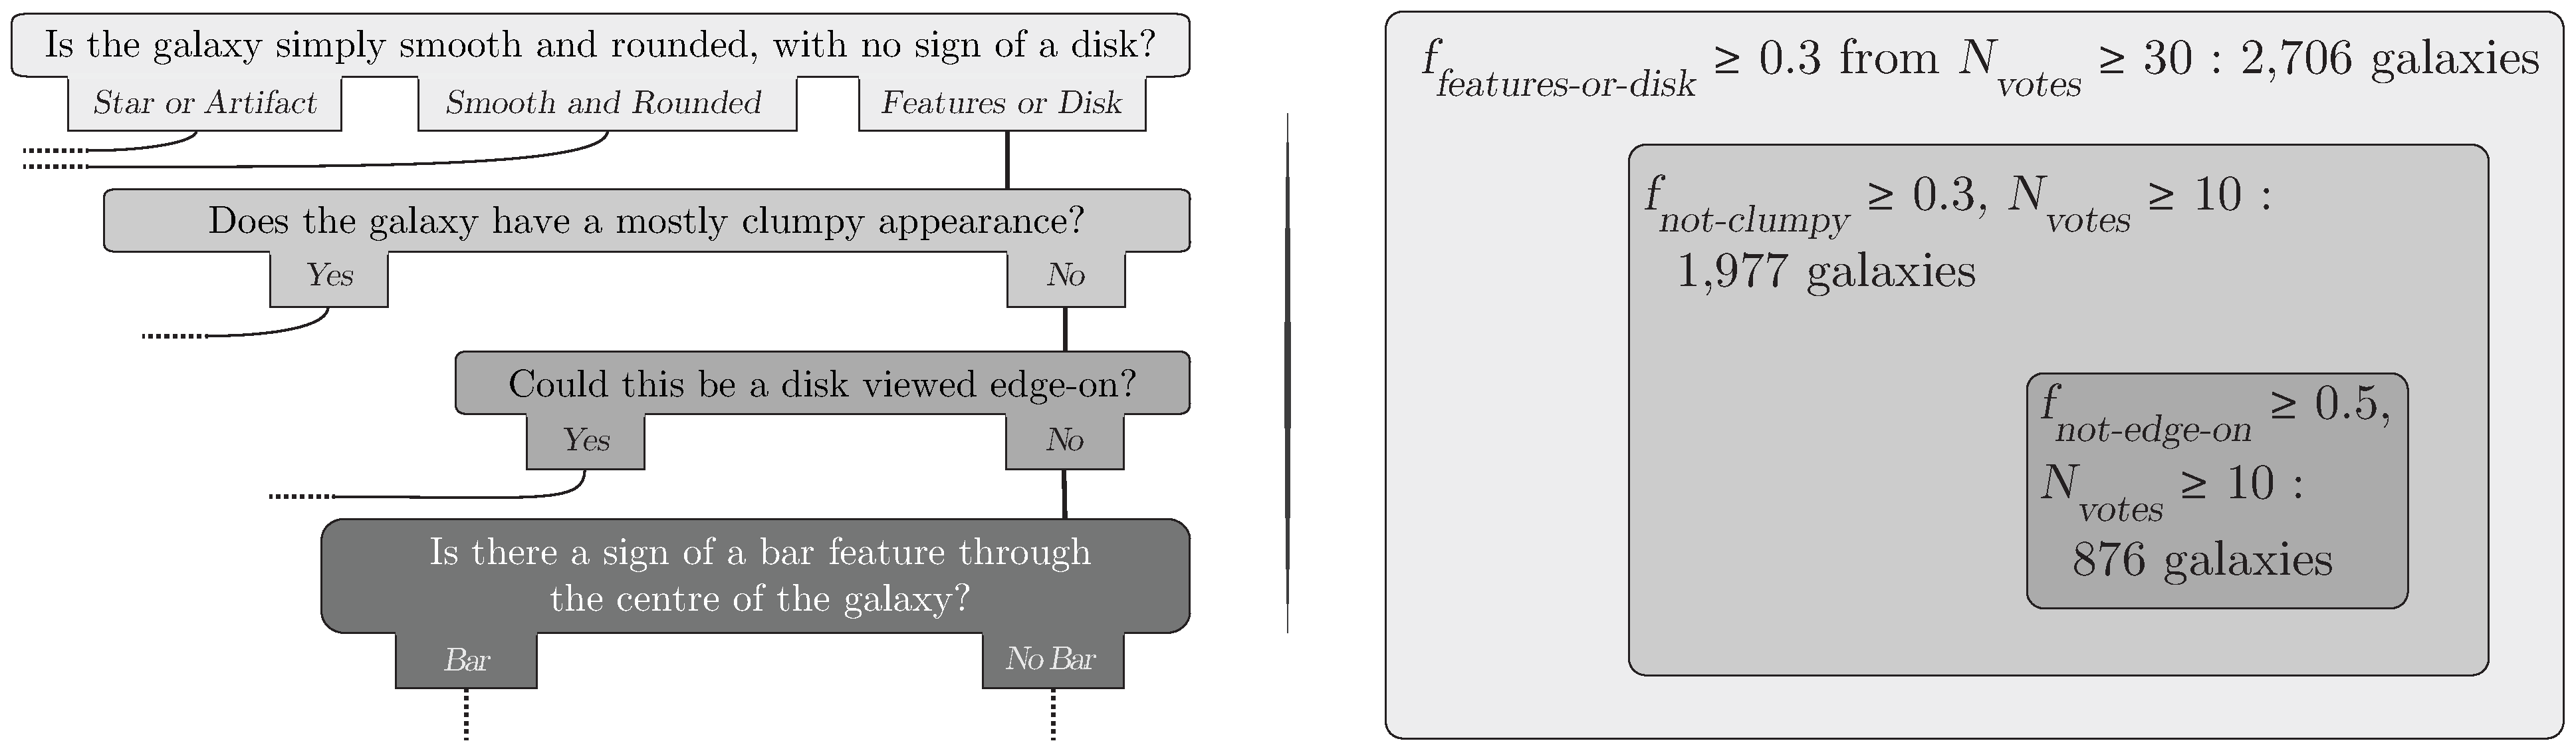
\includegraphics[scale=0.273]{tree_part_with_selection.eps}
\caption{
\emph{Left:} Partial Galaxy Zoo-CANDELS classification tree, starting with the first question (top) and leading to the bar feature question. There are 17 questions total in the tree; the bar question is a 4th-tier task. \emph{Right:} Selection of the featured, not-edge-on disk galaxy sample (876 galaxies) in GZ-CANDELS; relative box areas are scaled to the sample sizes. This selection was made independently of restrictions on redshift or luminosity (a full description of the sample selection is given in Section \ref{sec:sample}). Eight independent classifiers subsequently examined each of the 876 disk galaxies for evidence of a bar. 
%{\notek Great diagram. Include the final luminosity-limited disk sample?} {\notebsm I figured this was for the morphological selection only, as the redshift and L cuts are a separate step.}
}
\label{fig:sampleselection}
\end{figure*}
%%%%% END FIGURE %%%%%


\subsection{Redshifts}\label{sec:z}

Each of the fields covered by CANDELS data has considerable ancillary data from previous and ongoing work. We assemble photometric and spectroscopic redshifts from the available literature. For galaxies in the COSMOS field, we combine spectroscopic redshifts from the zCOSMOS project \citep{lilly07} with photometric redshifts from COSMOS \citep{ilbert09} and from the NEWFIRM medium-band survey \citep{whitaker11}. In the GOODS-South field, we use the catalog of \citet{cardamone10b}, who added photometric redshifts based on deep broad- and medium-band data from MuSYC \citep{gawiser06} to available spectroscopic redshifts compiled from multiple sources \citep{yes,you,must,cite,them,all,dont,be,lazy}. In the UDS field, we use available spectroscopic \citep{ref1, ref2, ref3} and photometric \citep{mortlock13} redshifts, the latter of which make use of deep multi-wavelength coverage from UKIDSS as well as $J$ and $H$-band magnitudes from CANDELS \citep[similar to photometric redshifts calculated by, e.g.,][]{candelsphotozref}. Of the 49,555 galaxies originally included in Galaxy Zoo-CANDELS, 46,234 currently have spectroscopic (2,886) or photometric (43,348) redshifts. Where available, agreement between spectroscopic and photometric redshift is generally very good, with $\sigma_z/(1+z_{spec}) = 0.017$.

%%%%%%%photoz + specz comparison


\subsection{Sample Selection}\label{sec:sample}


%%%%% [FIGURE: Example images] %%%%%
\begin{figure*}
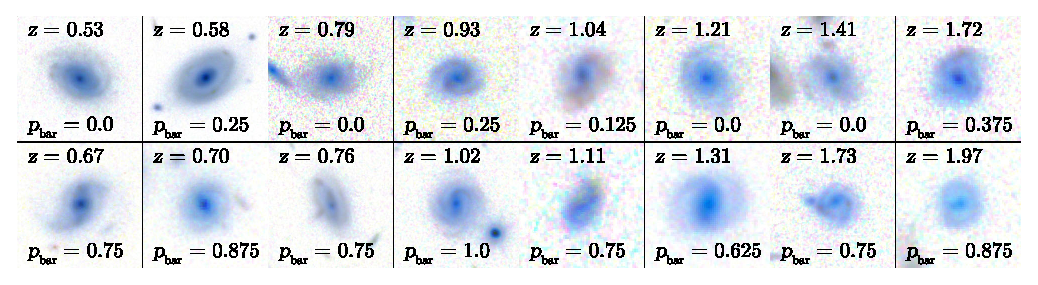
\includegraphics[scale=1.0]{barfig_3.eps}
\caption{
Examples of disk galaxies in GZ-CANDELS whose bar vote percentage $(p_{bar})$ is below (top row) and above (bottom row) the threshold for inclusion in the barred sub-sample.  {\notebsm To Do: you accidentally selected preferentially spirals. Don't.}
}
\label{fig:gals}
\end{figure*}
%%%%% END FIGURE %%%%%


A full reduction of the GZ-CANDELS classifications, resulting in a catalog of morphological votes for each galaxy, is ongoing. Here we use the raw vote percentages, which have been neither weighted nor debiased. The effects of using raw versus the reduced classifications are twofold. First, the unweighted votes are likely biased in the first question toward an excess of votes for ``Star or Artifact'' (see \citeauthor{willett13} \citeyear{willett13} for a discussion of how inconsistent votes are downweighted in Galaxy Zoo 2). Second, the effects of surface brightness dimming and loss of spatial resolution are not accounted for in the vote percentages, which is potentially a significant effect in a sample extending to $z \sim 2$ in the rest-frame optical.

To favour completeness in the final disk galaxy sample and to minimize the impact of the lack of user weighting, we employ a lower vote percentage threshold when selecting ``featured'' galaxies compared to thresholds using weighted data. We select as ``featured'' galaxies those where at least 30\% of votes (out of at least 30 volunteers total) were registered for ``Features or Disk''. This selects 2,706 featured galaxies. After the first question, the user weighting used by previous Galaxy Zoo data reductions affects vote percentages by typically no more than a few percent; we therefore expect the lack of weighting to have little to no systematic effect on additional vote percentages. 
%{\notek I hope that's true, but it really hasn't been shown explicitly. Something for BDS, KW, SB et al. to work on.} {\notebsm I looked at this in some detail when I started playing with GZH results. Once you get past the first question the difference in any given vote percentage between using weighted and unweighted is typically less than $\sim 3$\%.}

Subsequent to the featured galaxy selection, we select a sub-sample where at least 30\% of volunteers (where a minimum of 10 answered the question) registered a vote for ``no'' to the question ``Does the galaxy have a mostly clumpy appearance?'' in order to remove galaxies whose features do not clearly include a disk; this selection removes 729 clumpy galaxies in total. We include this selection in order to consider each branch of the classification tree that leads to the bar-feature question; however, we note that were we to ignore the clump-threshold criterion completely, this would only cause contamination of the final ``featured'' sample at the 1\% level, due to the subsequent selection criteria. Our qualitative results are thus not sensitive to the specific choice of clumpy threshold between $0.1 \leq p_{\mathrm not-clumpy} \leq 0.6$.

%%%%% [FIGURE: Volume-limited sample] %%%%%
\begin{figure}
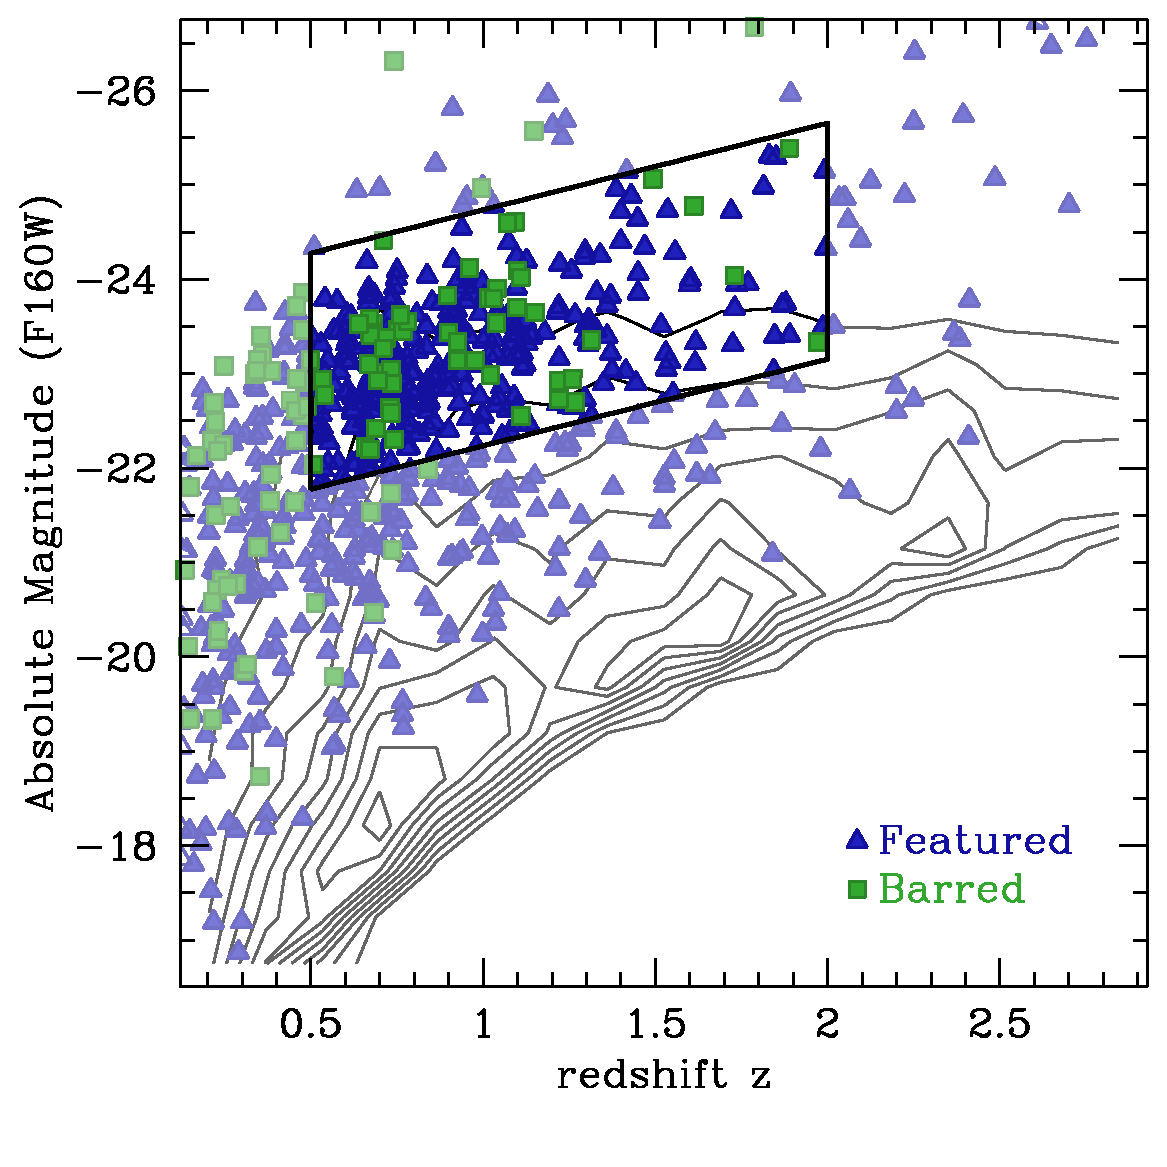
\includegraphics[scale=0.41]{Mag_z_contours.eps}
\caption{
Absolute $H$-band magnitude versus redshift for all sources with $H < 25.5$ (contours in steps of 10\%) and 876 ``Featured'' not-edge-on disks (blue triangles), of which 123 galaxies show clear evidence of a bar (green squares). To facilitate comparison between lookback times, avoid biases due to surface-brightness dimming when calculating bar fractions, and ensure all observed $H$-band flux is redward of the 4000-\AA\ break, we select sub-samples within the same region of the evolving galaxy luminosity function \citep{marchesini12} and $0.5 \leq z \leq 2$ (parallelogram). Within this region there are 370 not-edge-on disk galaxies, 56 of which have clear evidence of bars.
}
\label{fig:mag_z}
\end{figure}
%%%%% END FIGURE %%%%%



Further, we also require that 50\% of volunteers (of at least 10) registered a vote for a disk galaxy that is ``not-edge-on''.
This threshold choice is higher to reflect a more conservative requirement that a bar always be detectable in the sample of disk galaxies (though the thresholds used to select disk features are less strict to slightly favour completeness).\footnote{The discussion in Section \ref{sec:results} assumes the bar fraction is the same in edge-on galaxies as face-on galaxies; we also note that an application of the results to include clump-dominated galaxies requires a similar assumption.} This selects a sample of 876 featured disk galaxies from which a bar may be identified, if it exists. Figure \ref{fig:sampleselection} shows a visual representation of this sample selection, from which a further sub-sample of barred galaxies may be identified. However, approximately 20\% of these 876 galaxies received less than 10 raw votes \emph{total} for the question ``Is there any sign of a bar feature through the centre of the galaxy?'', a consequence of the broad initial selection of featured galaxies and the multiply-branched nature of the classification tree. Because of the lower number of votes per galaxy in the 4$^{\rm{th}}$ tier of the classification tree (the position of the bar question), within the featured sample the raw bar fractional vote is statistically useful, but uncertain for individual galaxies.

We therefore elected to supplement the volunteer data with visual classifications from the Galaxy Zoo science team to select the sub-sample of barred disk galaxies. Eight of the authors\footnote{BDS, TM, KWW, WCK, MR, KLM, RS, EC} inspected each of the 876 featured disk galaxies for evidence of a bar; these votes were unanimous approximately 60\% of the time, either for a bar feature (23 galaxies) or no bar (512 galaxies). Among galaxies where the science team voted unanimously that a bar is present, the mean volunteer bar vote percentage is  $0.65 \pm 0.15$. Among galaxies where the science team was unanimous that a bar is \emph{not} present, the mean volunteer bar vote percentage is $0.11 \pm 0.11$. The science team and volunteer bar vote percentages generally correlate, although the low number of volunteer votes for many objects means the dispersion in the correlation is high. Following vote percentage thresholds used in previous studies \citep[this method has been shown to select strong bars;][]{masters11a,willett13,melvin14}, we mark a galaxy as barred if at least half of the science-team classifiers indicated the presence of a bar ($p_{bar} \geq 0.5$). 
%We also note that this vote fraction threshold is statistically identical to a vote threshold of 45\% among volunteer votes (123 barred galaxies from science team votes vs. 121 from raw volunteer votes), but the overlap is only approximately 70\%.
%

The absolute $H$-band magnitudes in the sample are plotted as a function of redshift in Figure \ref{fig:mag_z}. Of the featured not-edge-on (and barred) galaxies, 525 (61) have redshifts between $0.5 \leq z \leq 2.0$. Within this redshift range, all flux collected by the WFC3 $H$ band is redward of the 4000-\AA\ break. Examples of barred and unbarred galaxies are shown in Figure \ref{fig:gals}.

To minimize any bias caused by surface-brightness dimming at higher redshifts, we additionally employ a conservative luminosity cut when examining bar fractions, choosing a minimum $H$ absolute magnitude of $-23.15$ at $z = 2$ (or approximately an apparent $H= 23.5$). This ensures that featured galaxies can be detected within the sub-sample at all $z < 2$. We note that this is brighter than the knee of the rest-frame-$V$-band luminosity function at this redshift \citep{marchesini12}. In order to examine similar populations across our entire redshift range, we use a varying luminosity cut based on selecting the same region of the evolving luminosity function \citep[corrected to observed $H$ band;][]{blanton07,marchesini12}: this selection is shown as a parallelogram shape in Figure \ref{fig:mag_z}. This final cut produces 370 featured, not-edge-on disk galaxies, of which 56 have strong bar signatures. We note that our results are robust to small variations in the redshift and luminosity thresholds chosen for the sample. For example, our qualitative result does not change if we use a fixed luminosity/stellar mass range.
% Note the high-L cut also helps avoid issues caused by the significant variations in completeness with magnitude across the various CANDELS fields, and even within individual CANDELS fields (e.g. GOODS-S has ERS, wide and deep). 

\subsubsection{Completeness corrections}\label{sec:completeness}

Given the depth of the CANDELS images (even those in the shallower ``wide'' fields) and the luminosity ranges considered here, the completeness of the final sample of featured, not-edge-on disk galaxies is unlikely to be affected by surface brightness dimming. Using Galaxy Zoo classifications is demonstrably reliable for selection of specific features \citep{darg10b,darg10a,masters11a,skibba12,casteels13,willett13,melvin14}, and all analysis here is concerned with large-scale strong galactic bars, which are less affected by surface brightness dimming or diminished resolution effects than smaller-scale or weaker features. In general, the selection is conservative with respect to detection of features, in the sense that both strong bars in particular and featured disks in general are unlikely to be missed.

However, it is possible that the selection described above could omit rotationally-supported disk galaxies with completely smooth light distributions (i.e., completely lacking in ``features''). As such galaxies would not contain bar features, they would preferentially bias the bar fractions discussed in Section \ref{sec:results} below to higher-than-actual values. This possible source of bias is not addressed by the conservative selection with respect to inclusiveness of features described above.

To correct for this possible bias, we examine the population of  ``smooth'' galaxies (that is, those where fewer than 30\% of votes from at least 30 total were registered for ``Features or Disk'' and fewer than 30\% of volunteers selected ``Star or Artifact'') within the luminosity and redshift selections described above. We assume this set of featureless galaxies contains a population of rotationally supported circular disk galaxies which are randomly oriented on the sky. We constrain the maximum possible fraction of disks within the featureless sample by assessing the highest fraction of the observed axis ratios within the featureless galaxies that is consistent with this population of randomly oriented disks. This fraction is $\approx 19\%$ for the full sample, and generally increases with redshift between 15\% and 25\%.

In the following analysis, we correct for this incompleteness factor by adding the maximum number of featureless, not-edge-on galaxies that may be disks to the total number of featured, not-edge-on disk galaxies in each redshift bin. Given the inclusive sample selection, the maximal correction for missed disk galaxies, and the lack of correction for possible contamination of non-disks in the sample, the bar fractions discussed below may be taken to be conservative lower limits.



%%%%%%%%%%%%%%%%%%%%%%%%%%%%%%%%%%%%%%%%%%%%%%
%
%
\section{Results: Bar fractions}\label{sec:results}
%
%
%%%%%%%%%%%%%%%%%%%%%%%%%%%%%%%%%%%%%%%%%%%%%%

The fraction of disk galaxies with visually identified strong bars between $0.5 \leq z \leq 2$ is $\sim 10\%$, a figure that is robust to moderate changes in luminosity ranges or vote fractions for detected features, lack of clumpiness, disk inclination angle, and strong bar features. Figure \ref{fig:barfrac} shows the bar fraction with lookback time, from $t_{lb} = 5.0$~Gyr ($z = 0.5$) to 10.2~Gyr ($z=2.0$). The sample encompasses the same subset of the galaxy luminosity function relative to the evolving $L^*$; the conservative selection to ensure detectability of features (or lack thereof) to $z = 2$ means the galaxies examined here are all brighter than $L^*$ at their epoch. 

Within this sample, and given the uncertainties, the bar fraction is consistent with zero evolution between $1 < z < 2$. Many studies of the bar fraction at $z \lesssim 1$ find that the bar fraction does evolve, though these findings are not unanimous \citep{abraham96,abraham99,jogee04,d_elmegreen04b,d_elmegreen05,sheth08,cameron10,melvin14}. Although the details depend on both the bar selection method being used and the properties of the galaxies themselves, disk galaxies are generally more likely to show strong bar features at lower redshift. Two independent studies of the full COSMOS-ACS sample \citep{sheth08,melvin14} show that the fraction of visually identified strong bars decreases with redshift, from approximately 35\% at $z = 0.2$ to 15\% at $z = 1$. 

%%%%% [FIGURE: Bar fractions and mags of sample] %%%%%
\begin{figure}
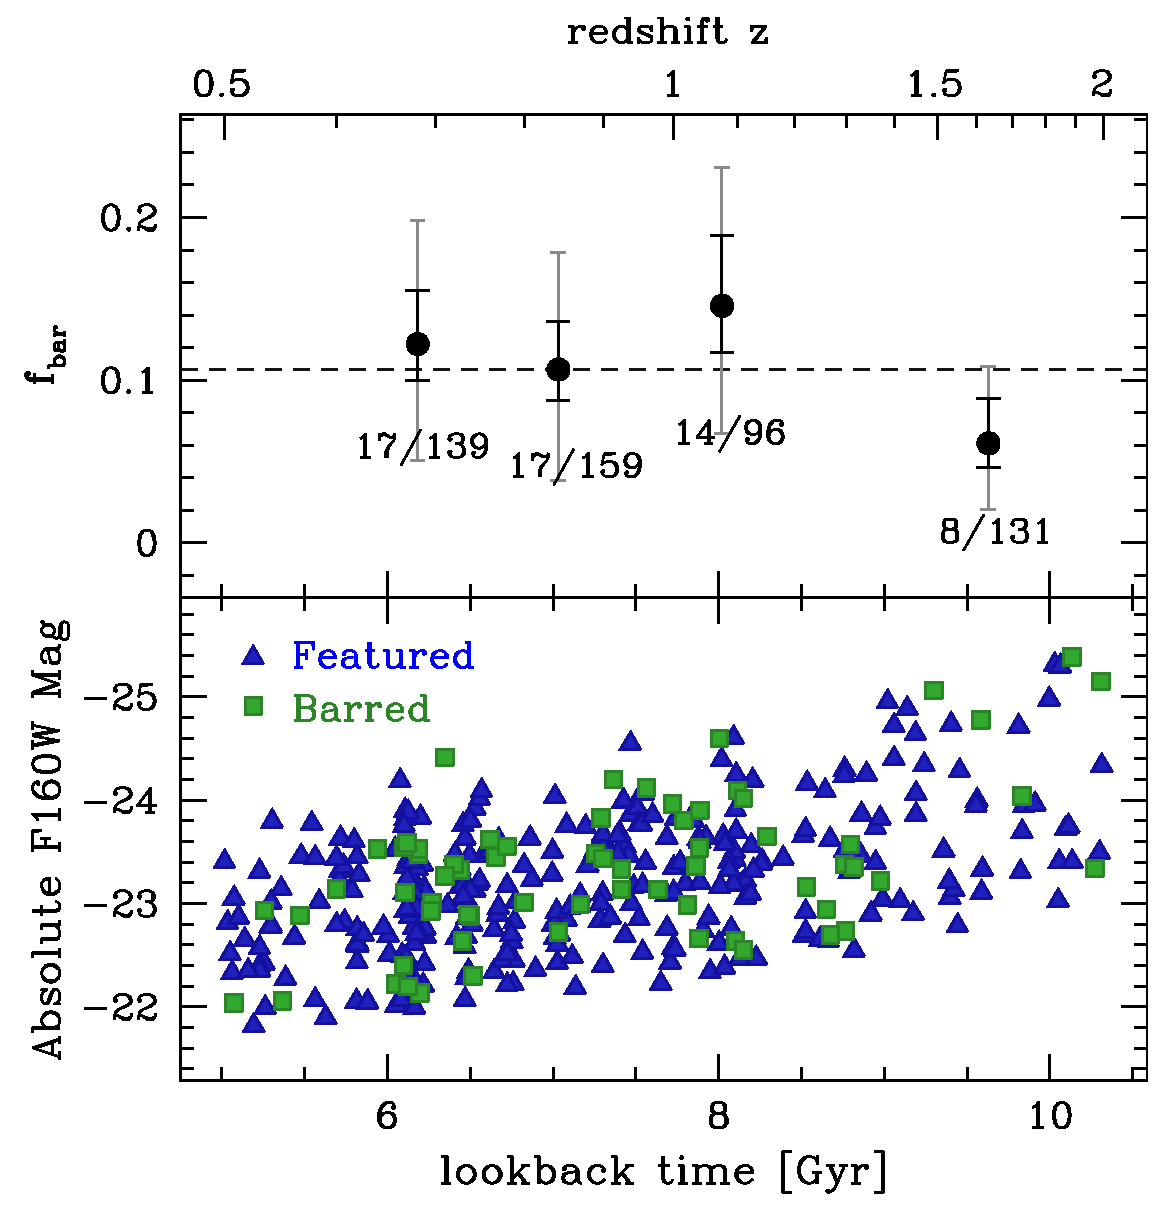
\includegraphics[scale=0.425]{barfrac_Mag_t.eps}
\caption{
\emph{Top panel:} Bar fraction versus lookback time. Error bars are 68\% (black) and 95\% (gray) Bayesian binomial confidence intervals \citep{cameron11}; within these confidence intervals, the bar fraction is consistent with no evolution from $0.5 \leq z \leq 2$. Bins were chosen to enclose similar lookback time intervals; the bar fraction across all bins ($10.7^{+1.5}_{-1.2}\%$) is shown as a dashed line. Black points include correction for incompleteness described in Section \ref{sec:completeness}; purple diamonds are the uncorrected fractions. \emph{Bottom panel:} absolute $H$-band magnitudes of the featured disk sample from which the fractions are drawn.
}
\label{fig:barfrac}
\end{figure}
%%%%% END FIGURE %%%%%


%%%%% [FIGURE: These results in context] %%%%%
\begin{figure}
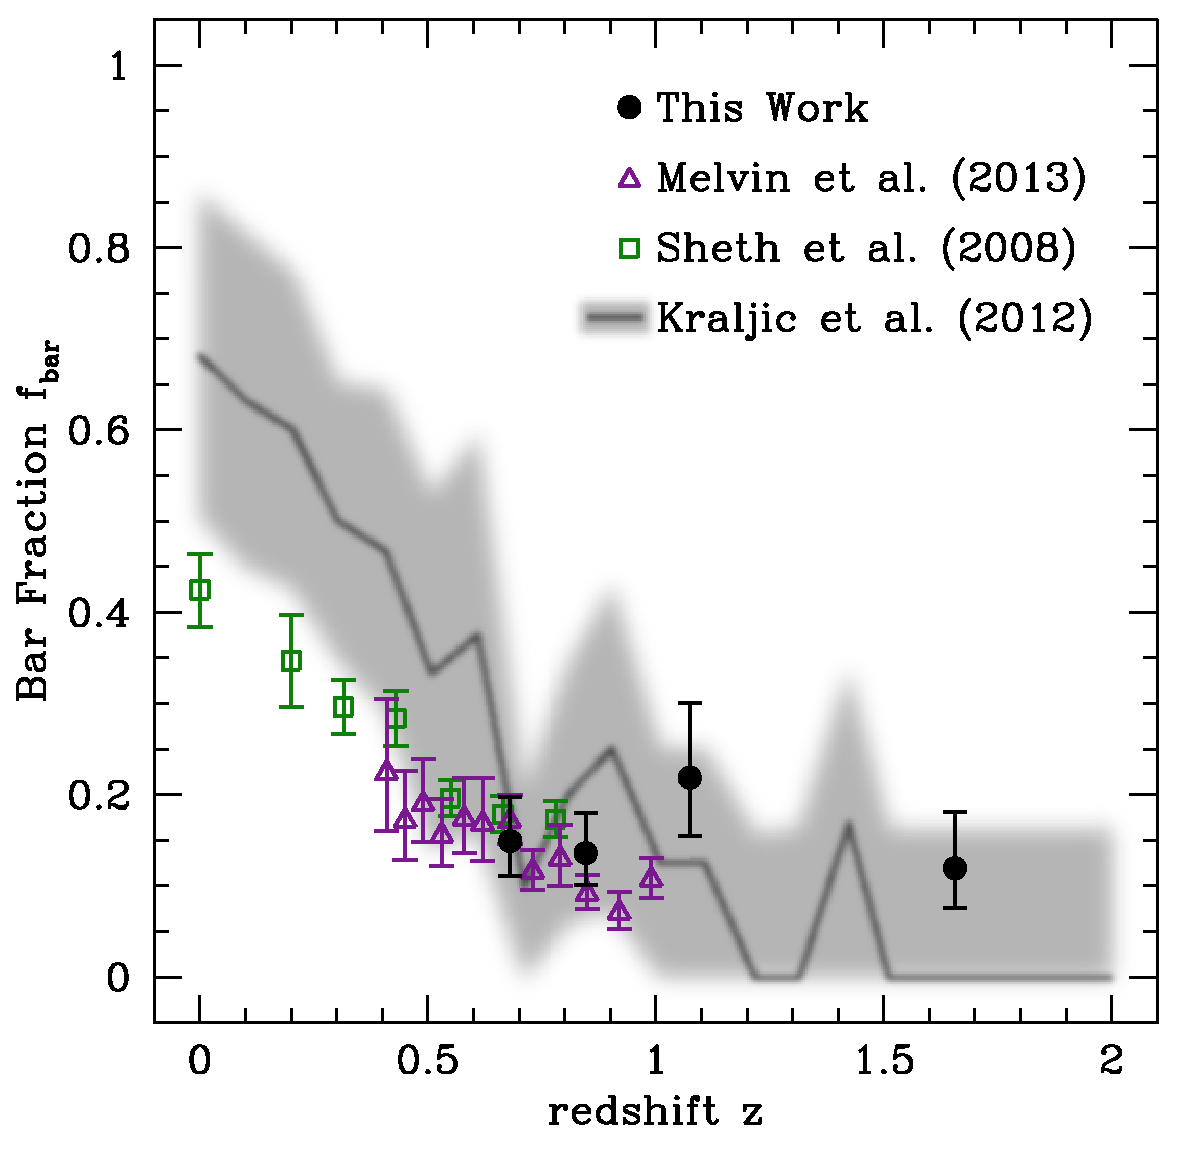
\includegraphics[scale=0.425]{barz_axes_withsims_strongbars.eps}
\caption{
Fraction of disk galaxies having a strong bar feature versus redshift, in the context of other work assessing visual strong bar fraction. 
All shading and error bars indicate Bayesian binomial confidence intervals \citep{cameron11}; 
the $1 \sigma$ error bars for the \citet[][Ma11, blue cross]{masters11a} and \citet[][dV91, red diamond]{RC3} fractions are smaller than the size of the points and are omitted.
At higher redshift, bar fractions in this work (black circles) at $z < 1$ are consistent with those of \citet[][S08, green squares]{sheth08}  and \citet[][Me14, purple triangles]{melvin14} despite differences in selection methods. 
\citet[][K12]{kraljic12} computed the fraction of strong bars to $z=2$ among disk galaxies that evolved to stellar masses $M_\ast \approx 10^{10-11} \mmsun $ (shaded region); the predicted bar fraction is consistent with that observed here within the uncertainties, although we note that differences between simulated and observed mass/luminosity ranges make direct quantitative comparisons more difficult. 
}
\label{fig:barfrac_context}
\end{figure}
%%%%% END FIGURE %%%%%


Figure \ref{fig:barfrac_context} shows the visually identified strong bar fraction versus redshift in the context of other work, both observational and theoretical. Within the redshift range where we overlap with other observational studies, the bar fraction is consistent. However, the bar fraction with redshift appears to flatten at $z > 1$. 

Using zoom-in cosmological simulations of 33 field and loose group galaxies, \citet{kraljic12} find that disk galaxies at $z \gtrsim 1$ 
% KLM comment: should this be "the progenitors of z ~ 0 disk galaxies, observed at z > 1"? BDS answer: in this case the plot shows the progenitors that are also disks at z > 1. But yes, all are progenitors of disk galaxies -- it's just not the full Kraljic sample.
are generally too dynamically hot to become unstable to bar formation; this manifests itself as a decreasing bar fraction with increasing redshift. Although the quantitative bar fractions in their simulations depend on the threshold used to define a bar feature, the fraction of disk galaxies hosting bars drops to zero, or near zero, by any definition they use \citep[Figure \ref{fig:barfrac_context} shows their standard ``strong bar'' definition, which is the closest to observational samples defined by visual classifications such as those here and in previous work;][]{masters11a,willett13,melvin14}. This initially appears inconsistent with our results showing a low, but non-zero, bar fraction. However,  due to the very small number of simulated galaxies in \citeauthor{kraljic12} that are disk galaxies at $z > 1$, a complete lack of bar feature detection within the subset of their sample identified as disk galaxies does not directly predict a $0\%$ bar fraction. Given that the normal approximation (used in that study) systematically underestimates proportional confidence errors when the true population fraction approaches 0 or 1, especially for small sample sizes, we have re-calculated the uncertainties quoted in \citeauthor{kraljic12} using a Bayesian approach to compute binomial confidence intervals \citep{cameron11}. Given this approach, the lack of detection of bars at $z > 1.5$ in the simulations is consistent with a bar fraction of up to $\approx 30$\% at these redshifts, within the 68\% confidence intervals. 

We also note that the galaxy masses and luminosities used in the simulations were on average lower %{\notek (How much?)} 
than those examined in this work, making a direct comparison to this work more difficult, as bar fraction also depends on stellar mass \citep{sheth08,melvin14}. \citeauthor{kraljic12} predict that massive disk galaxies will be more likely to form bars at higher redshift than lower mass disk galaxies due to higher-mass galaxies reaching dynamical maturity at earlier epochs. This is qualitatively consistent with our finding that the bar fraction at $z \sim 2$ may be as high as $12\%$ within $2 \sigma$ binomial uncertainties, but a direct and quantitative theoretical comparison to our observational result is currently not possible given available simulations. New simulations encompassing galaxies with higher stellar masses would help to advance this field further.

Our results agree with previous work that the main epoch of bar formation in the disk galaxy population begins at $z < 1$. However, bars are not completely absent even at $z \sim 2$: some disks at the masses probed by our sample are mature enough even by this epoch ($\sim 3-4$ Gyr after the Big Bang) to host a bar. 

Whether the bar features are analogous to long-lived bars in dynamically cold disks at lower redshift or are shorter-lived features triggered within dynamically warmer disks is unclear from examination of bar fractions alone. Examination of individual simulated galaxies by \citeauthor{kraljic12} indicates that bars formed at $z > 1.5$ tend to undergo shorter cycles of formation and destruction., and there is some evidence that short-lived grand design spiral features more commonly associated with mature disks can be triggered by interactions at $z > 2$ \citep{law12}.

 

Thus the incidence of bars in massive high-redshift disks may be due at least in part to galaxy interactions and mergers, combined with shorter bar lifetimes due to dynamically warmer disks. Minor galaxy mergers may dynamically heat a disk and destroy a bar, or they may trigger the formation of a bar, depending on the particulars of the interaction \citep{gerin90,berentzen03,berentzen04}. The relative likelihood of these contrasting end results, combined with the incidence of minor mergers among this population at $z \sim 2$, may combine to produce a net effect that stabilizes the bar fraction at $z \sim 10$\% during this epoch of galaxy assembly. 

{\notek That's intriguing. Can the GZ results say anything about the fraction of disks that look dynamically disturbed, either from volunteer data or re-examination by us? Maybe we could look at how $f_{odd}$ or $f_{merger}$ differs among barred and non-barred galaxies?} {\notebsm There's no longer an $f_{odd}$, but we do have the merger fraction and $f_{tidal}$; at least a first look is within scope and definitely a good idea.}

{\notebsm Have looked at merger votes and it's... intriguing, but hard to conclude anything. The highest-z stuff does seem to have a higher merger-or-tidal vote fraction, but it's not that conclusive. TO DO: write this more officially.}






%%%%%%%%%%%%%%%%%%%%%%%%%%%%%%%%%%%%%%%%%%%%%%
%
%  
\section{Summary}
%
%
%%%%%%%%%%%%%%%%%%%%%%%%%%%%%%%%%%%%%%%%%%%%%%

Using visual classifications of rest-frame optical \emph{HST} galaxy images from the ongoing Galaxy Zoo-CANDELS project, we examined for the first time the fraction of disk galaxies hosting a bar feature to $z \sim 2$ in order to trace the dynamical state of disks as early as $\sim 3$~Gyr after the Big Bang. We find that the bar fraction to $z \sim 1$ is consistent with previous studies using similar analysis methods. 

At $z > 1$, the bar fraction is approximately $10-20$\% and consistent with no evolution between $1 < z < 2$. This is qualitatively consistent with the predictions of zoom-in cosmological simulations, although further work is needed to determine whether simulations of disk galaxies with $L > L^*$ predict the same quantitative strong bar fraction at $z < 2$. 

That the bar fraction from $1 < z < 2$ appears to be small but constant among massive disk galaxies implies that massive disk dynamics do not rapidly change on average over this period. Further clarification may come in the future when additional detailed morphological classifications of deep $z \sim 2$ rest-frame optical galaxy images are available; future comparison with independent morphologies of the same galaxies  \citep{kartaltepe14} as well as additional simulations will help provide a more nuanced understanding of the underlying physical causes of this apparently stable bar fraction. 
  
%%%%%%%%%%%%%%%%%%%%%%%%%%%%%%%%%%%%%%%%%%%%%%
%
%
\section*{Acknowledgments}
%
%
%%%%%%%%%%%%%%%%%%%%%%%%%%%%%%%%%%%%%%%%%%%%%%

%The authors wish to thank to C. Peng for making \galfit\ publicly available, and for many enlightening discussions.  We also wish to thank R. Skibba, M. Williams, and the anonymous referee for thorough and constructive comments that helped us improve this manuscript.
%
TOPCAT \citep{taylor05} and an OS X widget form of the JavaScript Cosmology Calculator \citep{wright06} were used while preparing this paper. 
%
BDS gratefully acknowledges support from the Oxford Martin School, Worcester College and Balliol College, Oxford.
%
KS gratefully acknowledges support from Swiss National Science Foundation Grant PP00P2\_138979/1. 
%
TM acknowledges funding from the Science and Technology Facilities Council ST/J500665/1.
%
KWW and LF acknowledge funding from the UMN Grant-In-Aid program. 
%
\textbf{\noteb Please send your grant acknowledgments at your earliest convenience.}
%
% Old acknowledgments:
%Support for the work of KS was provided by NASA through Einstein Postdoctoral Fellowship grant number PF9-00069, issued by the Chandra X-ray Observatory Center, which is operated by the Smithsonian Astrophysical Observatory for and on behalf of NASA under contract NAS8-03060.
%
%ECM acknowledges support from the National Science Foundation through grant AST-0909063.
%
%SK acknowledges fellowships from the 1851 Royal Commission, Imperial College London, Worcester College, Oxford and support from the BIPAC institute at Oxford.
%
%KLM acknowledges funding from The Leverhulme Trust as a 2010 Early Career Fellow.
%
%SPB acknowledges receipt of an STFC Advanced Fellowship.
%
%RCN acknowledges STFC Rolling Grant ST/I001204/1 to ICG for �Survey Cosmology and Astrophysics�. 

The development of Galaxy Zoo was supported in part by the Alfred P. Sloan Foundation. Galaxy Zoo was supported by The Leverhulme Trust. 

This work is based on observations taken by the CANDELS Multi-Cycle Treasury Program with the NASA/ESA HST, which is operated by the Association of Universities for Research in Astronomy, Inc., under NASA contract NAS5-26555.

%This publication makes use of data products from the Wide-field Infrared Survey Explorer, which is a joint project of the University of California, Los Angeles, and the Jet Propulsion Laboratory/California Institute of Technology, funded by the National Aeronautics and Space Administration.

%Funding for the SDSS and SDSS-II has been provided by the Alfred P. Sloan Foundation, the Participating Institutions, the National Science Foundation, the U.S. Department of Energy, the National Aeronautics and Space Administration, the Japanese Monbukagakusho, the Max Planck Society, and the Higher Education Funding Council for England. The SDSS Web Site is http://www.sdss.org/.

%The SDSS is managed by the Astrophysical Research Consortium for the Participating Institutions. The Participating Institutions are the American Museum of Natural History, Astrophysical Institute Potsdam, University of Basel, University of Cambridge, Case Western Reserve University, University of Chicago, Drexel University, Fermilab, the Institute for Advanced Study, the Japan Participation Group, Johns Hopkins University, the Joint Institute for Nuclear Astrophysics, the Kavli Institute for Particle Astrophysics and Cosmology, the Korean Scientist Group, the Chinese Academy of Sciences (LAMOST), Los Alamos National Laboratory, the Max-Planck-Institute for Astronomy (MPIA), the Max-Planck-Institute for Astrophysics (MPA), New Mexico State University, Ohio State University, University of Pittsburgh, University of Portsmouth, Princeton University, the United States Naval Observatory, Yale University and the University of Washington. 
  
\bibliographystyle{mn2e}
\bibliography{refs}  


  
\end{document}
  
